%%%%%%%%%%%%%%%%%%%%%%%%%%%%%%%%%%%%%%%%%%%%%%%%%%%%%%%%%%%%%%%%%%%%%%%%
%                                                                      %
%     File: Thesis_Results.tex                                         %
%     Tex Master: Thesis.tex                                           %
%                                                                      %
%     Author: Andre C. Marta                                           %
%     Last modified : 21 Jan 2011                                      %
%                                                                      %
%%%%%%%%%%%%%%%%%%%%%%%%%%%%%%%%%%%%%%%%%%%%%%%%%%%%%%%%%%%%%%%%%%%%%%%%

\chapter{Validation and Experimental Results}
\label{chapter:results}


\section{Dataset Description}
\label{section:datasets}
In order to validate our proposal, we used two different real datasets from the healthcare field: the ALS and the Hepatitis datasets.

\subsection{ALS Dataset}
\label{subsection:als}

The ALS dataset\footnote{https://nctu.partners.org/ProACT/} includes information from over 8500 ALS patients who participated in industry
 clinical trials. The data include demographic, family and medical history, the patient’s history in terms of ALS symptoms,
 clinical and some laboratorial data. From these, we used a subset composed by the patients that had demographic data, had 
 performed Slow Vital Capacity exams, as well as measurements of their vitals, counting 13 variables: gender, age, height, 
 percentage of normal, subject liters (trial 1, 2 and 3), blood pressure (systolic and diastolic), pulse, respiratory rate,
 temperature and Weight. 

The outcome is a score that evaluates the state of the disease between 0 (severe) and 48 (normal), discretized into 
4 classes (aggregations of 12 points). The subset contains 578 patients, with 5\% for the 1st class, 22.3\% for the 2nd,
 29.1\% for the 3rd and 42.7\% for the 4th, and 0.88\% non-classified.

\subsection{Hepatitis Dataset}
\label{subsection:hepatitis}

The Hepatitis dataset was made available as part of the ECML/PKDD 2005 Discovery 
Challenge\footnote{http://lisp.vse.cz/challenge/CURRENT/}, it contains information about
 771 patients, and more than 2 million examinations between 1982 and 2001. Based on the work of \cite{Watanabe2003}
 the data was reduced to the most significant exams. In the end 17 variables were used: gender, age, birthdate, birth decade, 
 11 of the most significant exams (GOT, GPT, ZTT, TTT, T-BIL, D-BIL, I-BIL, ALB, CHE, T-CHO and TP) and the results from the
 active biopsies at the time of the exams (type, activity and fibrosis).

Fibrosis is the objective class and it is described by integer values between 0 (no-fibrosis) and 4 (most severe).
 The subset contains 488 patients and the following distribution of 
 classes: 2.05\% of 0, 45.9\% for 1, 21.35\% for 2, 15.19\% for 3 and 15.40\% for 4.

-------------------------------------------------------------

\subsection{SEER Dataset}
\label{subsection:seer}

The SEER data was requested from the Surveillance, Epidemiology, and End Results (SEER) web site. The data is composed by 9 files where each 
one contains data related to a specific cancer (breast, colon, urinary, etc.). It is composed by variables that give socio-demographic and
 cancer specific information concerning an incidence of cancer. Each record represents a particular patient-tumor pair within a registry. Each
 record is assigned a case number for each patient, and a unique record number for each specific tumor.



 \section{Validation Techniques}
\label{section:validation}

Both of the datasets have already been used successfully when performing the task of prognosis, the SEER data being use to predict patient 
survivability while the ALS data was used to predict disease’s progression. 

The reason to use 2 datasets describing different diseases, instead of just one, is to show the generalizability of our approach and hopefully
its similar results in both.

We will not be preprocessing any of the data, because that is not the objective of the proposed work. 

Our objective is to focus on finding a way to use the time dimension when per-forming prognosis, use a patients’ evolution over time, and with
that build a generalizable technique whose results are not so dependent on the data.

For these reasons, and because there are other works where these datasets have been used and preprocessed, \cite{Delen2005} \cite{Choi2009}
\cite{Lakshmi2013} , we can base our work on their results and use most of our time on the actual task in hand. 

Having the two datasets and the model built, the usual classification metrics will be used, like accuracy, sensitivity and specificity.

Accuracy is the ratio of correct classifications over all the cases,

\begin{equation}
Accuracy=\frac{TP+TN}{P+N}
\label{eq:accuracy}
\end{equation} 

with TP the number of true positives, TN the number of true negatives, and P and N the number of positive and negative cases, respectively.
While sensitivity, also called true positive rate, is the ability of the model to identify positive cases, in other words this metric shows the overall percentage of positive classifications.


\begin{equation}
Sensitivity= \frac{ TP}{TP+FN}
\label{eq:sensitivity}
\end{equation} 

Because only measuring the ability to identify the positive cases is useless (a system that always classified something as positive would have a sensitivity of 1), we also use specificity. Similarly, specificity measures the ability of the system to identify the negative cases.

\begin{equation}
Specificity= \frac{ TN}{FP+TN}
\label{eq:specificity}
\end{equation} 

Because the use of time is the cornerstone of this work it is also needed to see if it was actually relevant, to do this we will look for the use of temporal patterns in the model created and their relevance in the decision process, i.e. if the model is a decision tree the closer to the root this temporal pattern rules are the more relevant they are in the decision and those showing the importance of time in this matter.



\section{Experimental Results}
\label{section:results}


\subsection{Diagnosis Model}
\label{subsection:diagnosis}

As a baseline for comparison with the proposed approaches we used two models. \emph{BaselineSingleObservation} is a diagnostic model
 where a single observation in time is used to perform the prognosis. In other words, the state of a patient at instant n is
 used to predict his class at instant $n+1$. On the other hand, \emph{BaselineMultipleObservation} instead of using a single observation,
 uses multiple observations: all information is used here to predict the class at instant $n+1$.

A collection of techniques were used with these models, with both achieving similar results: the precision ranged between 40\% and 55\%,
 depending on the dataset, technique and number of time points used, as seen in \ref{fig:baselinesingle} and \ref{fig:baselinemulti}.
 
 \begin{figure}
  \begin{subfigmatrix}{2}
	\subfigure[ALS]{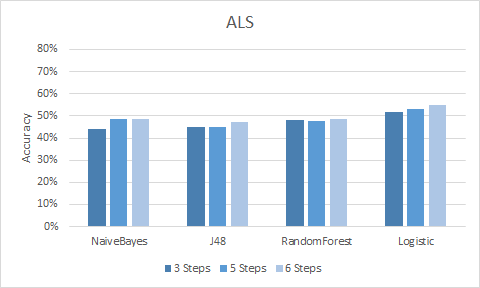
\includegraphics[width=0.49\linewidth]{Figures/base_single_als_tree.png}}
	\subfigure[Hepatitis]{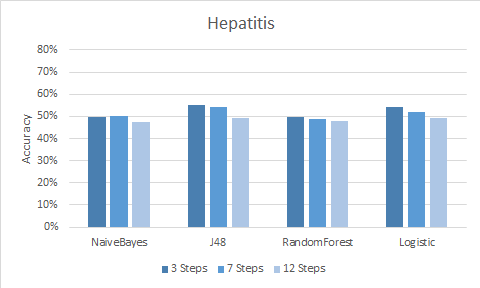
\includegraphics[width=0.49\linewidth]{Figures/base_single_h_tree.png}}
  \end{subfigmatrix}
  \caption{BaselineSingleObs precision (several classifiers and number of observations).}
  \label{fig:baselinesingle}
\end{figure}

 \begin{figure}
  \begin{subfigmatrix}{2}
	\subfigure[ALS]{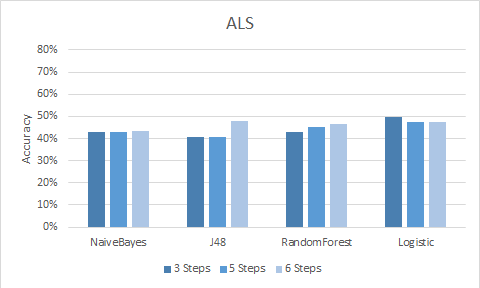
\includegraphics[width=0.49\linewidth]{Figures/base_multi_als_tree.png}}
	\subfigure[Hepatitis]{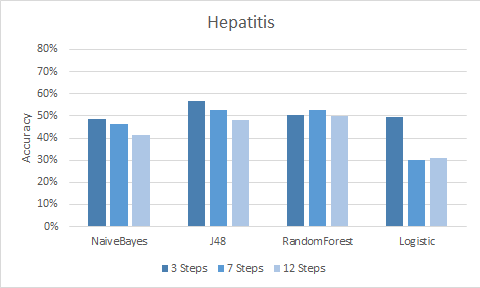
\includegraphics[width=0.49\linewidth]{Figures/base_multi_h_tree.png}}
  \end{subfigmatrix}
  \caption{BaselineMultipleObs precision (several classifiers and number of observations).}
  \label{fig:baselinemulti}
\end{figure}



\subsection{Regression Techniques}
\label{subsection:regresion}

Because of the differences of the various datasets, some numeric and some nominal, different regression techniques have been applied
 in the estimation phase of this work, namely linear regression for the numeric datasets and logistic regression for the nominal.
  
\subsubsection{Estimation Models}
\label{subsubsection:estimation_regression}

The results with the univariate and multivariate estimation models for the ALS dataset, numeric, can be seen in 
\ref{fig:estimationals}. This models were built using linear regression
 as previously said. Both estimation models were applied using a different number of observations, and the previous.
 Because the dataset is numeric we evaluated our estimation by the error, distance, to the actual value at time $t_{n+1}$.
 Both the univariate and the multivariate estimation model presented an average estimation error of  around $9,4$. 
 \hl{, with features having errors as high as $25$ and as low as $0.35$.}
  
\begin{figure}
	\begin{subfigmatrix}{2}
	\subfigure[Univariate Estimation]{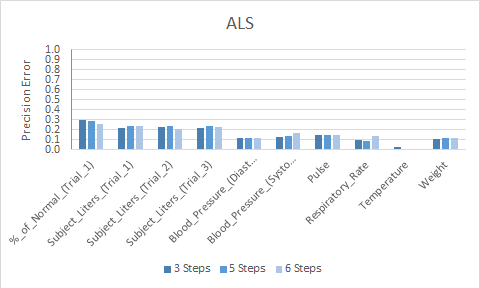
\includegraphics[width=0.49\linewidth]{Figures/estimation_single_als_reg.png}}
	\subfigure[Multivariate Estimation]{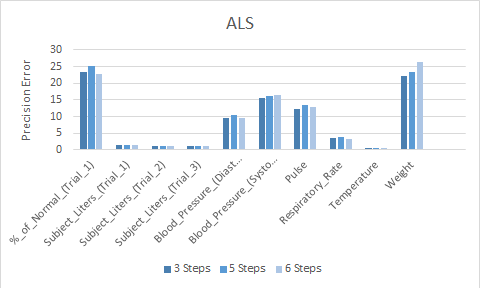
\includegraphics[width=0.49\linewidth]{Figures/estimation_multi_als_reg.png}}
  \end{subfigmatrix}
  \caption{Impact of the number of observations on the precision of the linear regression estimation models for each variable, in the ALS dataset.}
  \label{fig:estimationals}
\end{figure}

We can also see in \ref{fig:estimationlogh} the results of using Logistic Regression on the
 Hepatitis dataset. In both cases the average precision of estimation rounded the 80\% range, with the multivariate model being consistently
 a bit worse the the model that uses a single variable.
 
 \begin{figure}
	\begin{subfigmatrix}{2}
	\subfigure[Univariate Estimation]{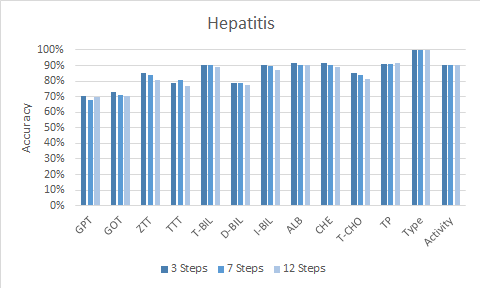
\includegraphics[width=0.49\linewidth]{Figures/estimation_single_h_log.png}}
	\subfigure[Multivariate Estimation]{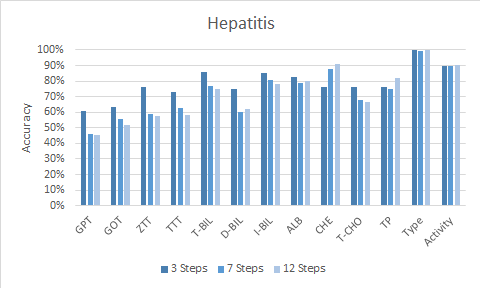
\includegraphics[width=0.49\linewidth]{Figures/estimation_multi_h_log.png}}
  \end{subfigmatrix}
  \caption{Impact of the number of observations on the precision of the logistic regression estimation models for each variable, in the hepatitis dataset.}
  \label{fig:estimationlogh}
\end{figure}


In \ref{fig:estimationtimeregression}, we can see the performance analysis, in milliseconds, of the estimation phase, divided by execution time 
per feature per feature. Its important to note that no significant difference was noticed between the univariate and multivariate estimations 
when using linear regression. The same cannot be said about logistic regression where the overall estimation of the features on the multivariate
approach took about $(N steps \times 3)$ times more than the univariate.

\begin{figure}
  \begin{subfigmatrix}{2}
	\subfigure[ALS - Linear Regression]{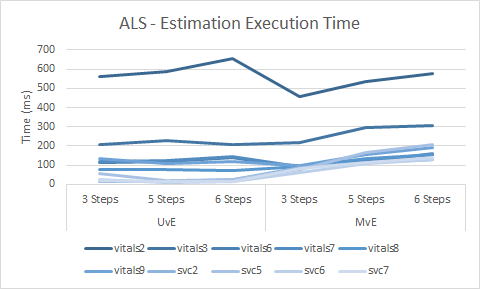
\includegraphics[width=0.49\linewidth]{Figures/time_estimation_linear_als.png}}
	\subfigure[Hepatitis - Logistic Regression]{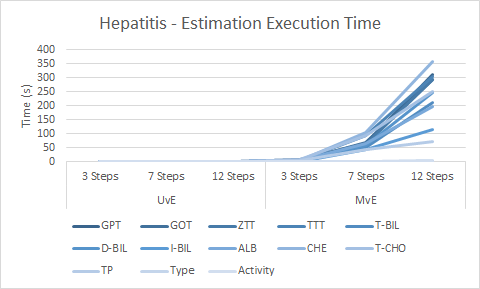
\includegraphics[width=0.49\linewidth]{Figures/time_estimation_logistic_h.png}}
  \end{subfigmatrix}
  \caption{Execution time of feature estimation in both datasets using regression techniques.}
  \label{fig:estimationtimeregression}
\end{figure}

\subsubsection{Prognosis Results}
\label{subsubsection:prognosis_regression}

The overall prognosis precision achieved by using different techniques on our approaches, with the predictions achieved by using regression 
techniques, can be seen in \ref{fig:precisionregression}. 

\ref{fig:impactregression} shows the relation between the number of observations and the final precision of the prognosis, using both, UvE and MvE
 estimation models, and a variety of techniques.

 \begin{figure}
  \begin{subfigmatrix}{2}
	\subfigure[ALS - linear regression estimations]{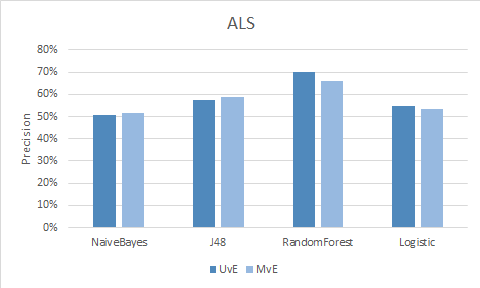
\includegraphics[width=0.49\linewidth]{Figures/precision_als_reg.png}}
	\subfigure[Hepatitis - logistic regression estimations]{\includegraphics[width=0.49\linewidth]{Figures/precision_h_log.png}} %grafico Hepatiti logistic
  \end{subfigmatrix}
  \caption{Precision of different models.}
  \label{fig:precisionregression}
\end{figure}

 \begin{figure}
  \begin{subfigmatrix}{2}
	\subfigure[ALS - linear regression estimations]{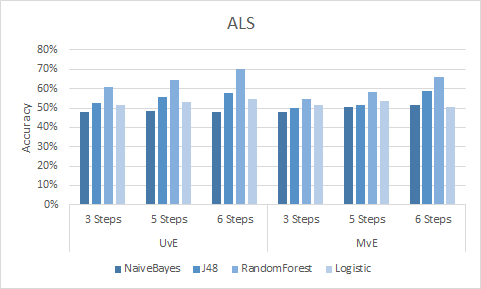
\includegraphics[width=0.49\linewidth]{Figures/impact_als_reg.png}}
	\subfigure[Hepatitis - logistic regression estimations]{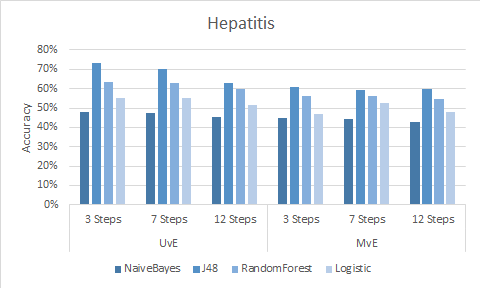
\includegraphics[width=0.49\linewidth]{Figures/impact_h_log.png}} %grafico Hepatiti logistic
  \end{subfigmatrix}
  \caption{Impact of the number of observation on prognosis models.}
  \label{fig:impactregression}
\end{figure}
 


 \subsection{Decision Tree}
\label{subsection:dt}

In this section, J48 was used as the estimation technique. Because J48 cannot handle numeric classification
 this technique was only used on the hepatitis dataset and the results were as follows.

\subsubsection{Estimation Models}
\label{subsubsection:estimation_dt}

Before, assessing the results of our prognosis approach, we evaluate the impact of the number of observations used, on the 
quality of the estimations made through the two estimation models proposed.

Since ALS observations are described by numerical variables and Hepatitis by nominal variables, we measured the prediction
 error (the distance from the predicted to the target value) and the number of correct predictions, respectively.

\ref{fig:estimationtreeh} shows the results with univariate and multivariate estimation models,
 respectively. Both estimation models were applied using a different number of observations, and the previous. 
 
\begin{figure}
  \begin{subfigmatrix}{2}
	\subfigure[Univariate Estimation]{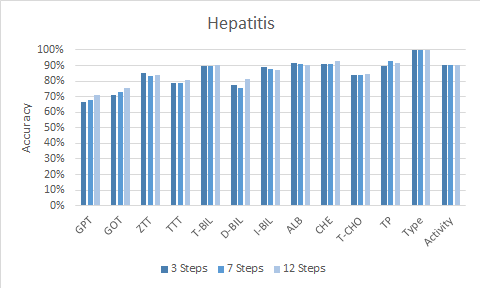
\includegraphics[width=0.49\linewidth]{Figures/estimation_single_h_tree.png}}
	\subfigure[Multivariate Estimation]{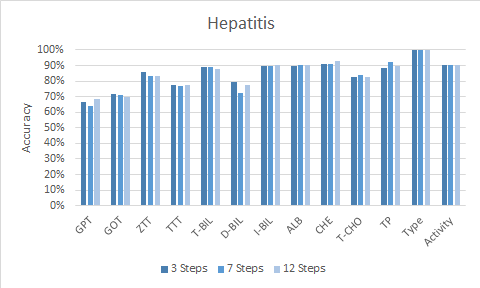
\includegraphics[width=0.49\linewidth]{Figures/estimation_multi_h_tree.png}}
  \end{subfigmatrix}
  \caption{Impact of the number of observations on the precision of the decision tree estimation models for each variable using both univariate and multivariate models.}
  \label{fig:estimationtreeh}
\end{figure}
 
Both models reach similar levels of accuracy, with quite good results for the majority of the Hepatitis variables
 (above 80\%). It is interesting that there is a slight trend to increase the accuracy as the number of observations get higher.

Despite our expectations, it seems that there is no improvement on using multivariate-based estimation.

In \ref{fig:estimationtimetree}, we can see the performance analysis, in milliseconds, of the estimation phase using decision 
trees, divided by execution time per feature.

It is important to note that even though the estimation using logistic regression had similar results (\ref{fig:estimationlogh}), when looking into to the precision of the estimation, it took much much longer to estimate those results
 ($3\times$ more in the the fastest case and $800\times$ more in the slowest, \ref{fig:estimationtimeregression} ).

\begin{figure}
  \centering
  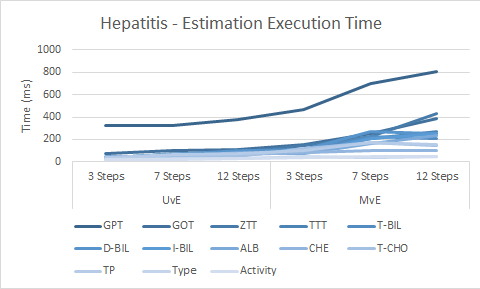
\includegraphics[width=0.75\textwidth]{Figures/time_estimation_tree_h.png}
  \caption{Execution time of feature estimation in the hepatitis dataset using decision trees.}
  \label{fig:estimationtimetree}
\end{figure}

\subsubsection{Prognosis Results}
\label{subsubsection:prognosis_dt}

The overall prognosis precision achieved by using different techniques on our approaches can be seen in \ref{fig:precisiontree}. The improvements 
on the precision of our approach are always present when compared to the ones achieved by baseline models 
(see \ref{fig:baselinesingle} and \ref{fig:baselinemulti}). In Hepatitis dataset the improvements round about 20\%.

\ref{fig:impactobservationstree} shows the relation between the number of observations and the final precision of the prognosis, using both, UvE and MvE
 estimation models, and a variety of techniques. It is interesting to note that the higher number of observations become prejudicial
 to the UvE model, which means that the values from the long past do not help to estimate future values. 

Again there is no clear difference between both estimation models, but decision trees (through C4.5 algorithm – J48) always 
perform better than the other models. 

\begin{figure}
	\centering
  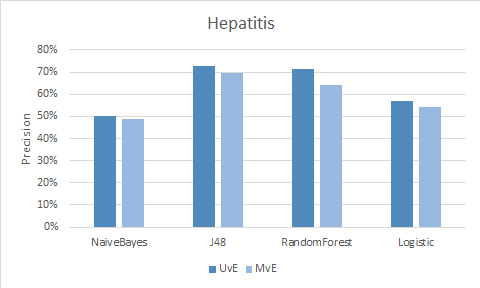
\includegraphics[width=0.49\linewidth]{Figures/precision_h_tree.png}
  \caption{Precision of different models using the decision trees estimations.}
  \label{fig:precisiontree}
\end{figure}

 \begin{figure}
	\centering
	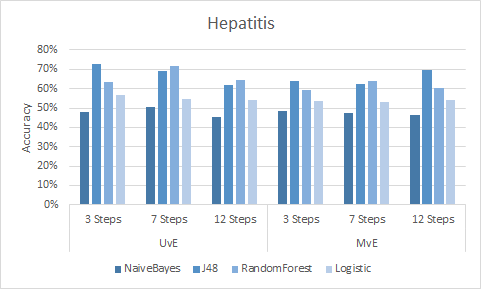
\includegraphics[width=0.49\linewidth]{Figures/impact_h_tree.png}
  \caption{Impact of the number of observation on prognosis models using the decision trees estimations.}
  \label{fig:impactobservationstree}
\end{figure}





\subsection{HMM}
\label{subsection:hmm}

In this final section, HMM were used in the estimation phase. Again like the C4.5 algorithm it doesn't handle
numeric classes so only the hepatitis dataset was used.

The HMMs we used had one state per time step used, so if we had a sequence with data from 7 time instances our HMM 
would have 7 states. All the probabilities distributions, $\lambda$, would then be initialized randomly and normalized 
so that the probability distribution equals to 1.

We would then train one HMM per class, using the Baum-Welch algorithm, which is used to adjust $\lambda$ to maximize the 
likelihood of the training set. The training set was composed by a subset of the data that had the specific class. 

The prediction phase was done by concatenating all the possible classes to the observed sequence and applying the forward
 algorithm with that sequence and the matching class HMM. The forward algorithm calculates the likelihood that the HMM 
 generated the sequence. The sequence with the highest likelihood was chosen and so the concatenated class was the estimation.

\subsubsection{Estimation Models}
\label{subsubsection:estimation_hmm}

\hl{Before, assessing the results of our prognosis approach, we evaluate the impact of the number of observations used, on the 
quality of the estimations made through the two estimation models proposed.}

\hl{Since ALS observations are described by numerical variables and Hepatitis by nominal variables, we measured the prediction
 error (the distance from the predicted to the target value) and the number of correct predictions, respectively.}

\ref{fig:estimationhmm} shows the results with univariate and multivariate estimation models,
 respectively. Both estimation models were applied using a different number of observations, and the previous. 
 
 \begin{figure}
  \begin{subfigmatrix}{2}
	\subfigure[Univariate Estimation]{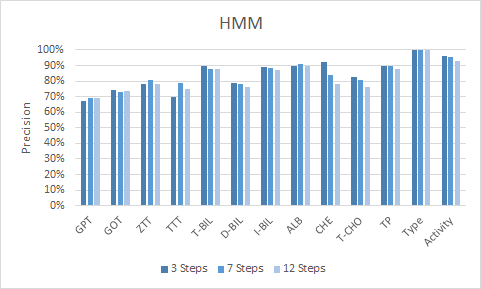
\includegraphics[width=0.49\linewidth]{Figures/estimation_single_h_hmm.png}}
	\subfigure[Multivariate Estimation]{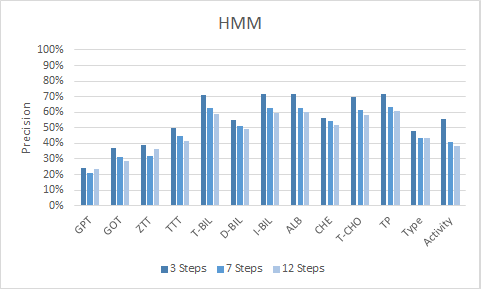
\includegraphics[width=0.49\linewidth]{Figures/estimation_multi_h_hmm.png}}
  \end{subfigmatrix}
  \caption{Impact of the number of observations on the precision of the HMM estimation models for each variable using both univariate and multivariate models.}
  \label{fig:estimationhmm}
\end{figure}
 
 In \ref{fig:estimationtimehmm}, we can see the performance analysis, in milliseconds, of the estimation phase using decision 
trees, divided by execution time per feature.

It is important to note that even though the estimation using logistic regression had similar results (\ref{fig:estimationlogh}
 and \ref{fig:estimationtreeh}), when looking into to the precision of the estimation, it took much much longer to estimate those results
 (\ref{fig:estimationtimeregression} and \ref{fig:estimationtimetree} ).
 
 \begin{figure}
  \centering
  \includegraphics[width=0.75\textwidth]{Figures/time_estimation_hmm_h.png}
  \caption{Execution time of feature estimation in the hepatitis dataset using HMMs.}
  \label{fig:estimationtimehmm}
\end{figure}

\subsubsection{Prognosis Results}
\label{subsubsection:prognosis_hmm}

% ------------------------------------------------------------



\subsection{Discussion}
\label{subsection:discussion}

Currently, medical practice is helped by a variety of computer-aided tools, dedicated to help physicians taking the most
 appropriate decisions. However, despite the importance of prognosis, it did not deserved dedicated tools, and in the majority 
 of situations, it has been addressed as a simple diagnosis problem, without exploring the temporality involved.

In order to mimic physicians practice, computer-aided prognosis should take into attention patients’ evolution, considering the 
different observations made along time. In this paper, we formalize both diagnosis and prognosis problems, making clear the
 differences between them, and propose a method to transform the prognosis into a diagnosis task, based on the composition
 of classification over the estimation of observation values. As described above, what distinguishes this approach, from what 
 is found in the literature, is the use of temporal dependencies of the data in order to estimate the future values of every 
 feature and with those values perform a diagnostic in the future. 
 
 
\cleardoublepage
